\documentclass[12pt]{article}

\usepackage{sbc-template}
\usepackage{graphicx,url}
\usepackage[utf8]{inputenc}
\usepackage[brazil]{babel}
\usepackage{fancyvrb}
\usepackage{caption}
\usepackage{enumerate}
\usepackage{subcaption}
\usepackage{listings}
\usepackage{color}
\renewcommand\lstlistingname{Código}
\def\lstlistingautorefname{Código}

\newcommand\slsh{\char`\\}

\usepackage{hyperref}
\hypersetup{
    colorlinks=true,
    linkcolor=cyan,
    filecolor=blue,      
    urlcolor=cyan,
    citecolor=cyan,
}
 
\sloppy

\title{Estudo relativo ao desempenho em função do consumo sobre alta demanda de dados em sistemas web desenvolvidos com \textit{Node.JS}}

\author{Marcos Renan Krul\inst{1}, Renato Cristiano Ruppel\inst{1}, Prof. Dr. Adriano Ferrasa\inst{1}}


\address{Universidade Estadual de Ponta Grossa (UEPG)
    \email{19022626@uepg.br, 19010426@uepg.br, ferrasa@uepg.br}
}

\definecolor{lightgray}{rgb}{.9,.9,.9}
\definecolor{darkgray}{rgb}{.4,.4,.4}
\definecolor{purple}{rgb}{0.65, 0.12, 0.82}

\lstdefinelanguage{JavaScript}{
  keywords={typeof, new, true, false, catch, function, return, null, try, async, catch, switch, var, if, in, while, do, else, case, break, const, for, await},
  keywordstyle=\color{blue}\bfseries,
  ndkeywords={class, export, boolean, throw, implements, import, this},
  ndkeywordstyle=\color{darkgray}\bfseries,
  identifierstyle=\color{black},.
  sensitive=false,
  comment=[l]{//},
  morecomment=[s]{/*}{*/},
  commentstyle=\color{purple}\ttfamily,
  stringstyle=\color{red}\ttfamily,
  morestring=[b]',
  morestring=[b]"
}

\lstset{
	language=JavaScript, 
	basicstyle=\small\ttfamily, 
	breaklines=true, 
	numbers=left, 
	numberstyle=\tiny\color{lightgray}, 
	stepnumber=1, 
	numbersep=8pt, 
	frame=single, 
	showspaces=false,
	showstringspaces=false,
	showtabs=false,
	captionpos=b, 
	xleftmargin=15pt, 
	xrightmargin=0pt, 
	tabsize=2, 
	commentstyle=\color{green!40!black}, 
	keywordstyle=\color{blue}, 
	stringstyle=\color{red}
}


\begin{document} 

\maketitle


\begin{resumo} 
O trabalho realiza um estudo sobre técnicas presentes na plataforma do \textit{Node.JS} para desenvolvimento de servidores \textit{web} 
que exijam processamento de grandes volumes de dados. Dentre os principais padrões de projeto, destaca-se a arquitetura orientada a eventos,
fortemente enraizada nos principais núcleos da plataforma, que, juntamente com as \textit{streams}, possibilita a leitura de arquivos 
com tamanho na ordem de \textit{gigabytes}. Serão criadas aplicações servidoras com o objetivo de testar a capacidade de lidar com altas 
demandas em aplicações web. Além disso, será avaliado como os recursos do servidor são utilizados ao lidar com a leitura e processamento 
de um arquivo de 1,65 GB. O resultado esperado é demonstrar que a arquitetura orientada a eventos é a solução mais eficaz para o 
desenvolvimento de aplicações web que lidam com grandes volumes de dados na plataforma Node.JS.
\end{resumo}


\begin{abstract} 
The work carries out a study of techniques present in the Node.JS platform for developing web servers that require processing large
volumes of data. Among the main design patterns, the event-driven architecture stands out, deeply rooted in the core of the platform, 
which, along with streams, enables the reading of files with sizes in the gigabytes range. Server applications will be created with the 
goal of testing the ability to handle high demands in web applications. Additionally, an evaluation will be conducted on how server 
resources are utilized when dealing with the reading and processing of a 1.65 GB file. The expected outcome is to demonstrate that the 
event-driven architecture is the most effective solution for developing web applications that deal with large volumes of data on the Node.JS platform.
\end{abstract}


\section{Introdução}

O desenvolvimento de aplicações \textit{web} bem como a migração de aplicações existentes para este ambiente,
é a realidade atual encontrada no mercado de \textit{software}. É considerado o meio mais utilizado
para comunicação e troca de informações atualmente, com mais de 2,5 quintilhões de \textit{bytes} de dados
carregados por diferentes serviços ofertados. Dentre outras, até janeiro de 2020, foram 
contabilizados cerca de 4,45 bilhões de usuários de \textit{internet} \cite{WEBUSAGE}. 
Existem benefícios que justificam esse comportamento, como facilidades em instalações e atualizações, 
alcance global instantâneo e alta portabilidade. Porém, sob outra perspectiva, apresentam-se questões 
críticas que devem ser analisadas antes de aderir à plataforma, como o desempenho em situações com 
alta demanda de dados.

O uso de \textit{Node.JS}, tecnologia em crescente uso e relevância no
desenvolvimento \textit{web}, justifica-se pelo fato de que esta permite uma abordagem de alta
performance e apresenta recursos para otimização e escalabilidade. Essa plataforma apresenta
bons resultados em casos que necessitem da persistência de centenas ou milhares de conexões
simultâneas, onde a comunicação é realizada com o envio de pequenos fragmentos do arquivo ao destino
\cite[p. 112]{EJSMONT}.

Aplicações como colaboração de documentos e tarefas, jogos e \textit{streaming} de vídeo, áudio e imagens
\cite{ZRHR} devem processar arquivos com tamanhos na ordem de \textit{gigabytes}. 
Contudo, existem limitações inerentes ao uso da plataforma \textit{web}, como o processamento de 
diversas requisições que exijam esses arquivos, tratamento de dados pela máquina 
cliente e os limites impostos pelas tecnologias escolhidas.

Para sobrepujar os problemas supracitados, existem técnicas desenvolvidas para a \textit{web} que buscam
atenuar os problemas de alta demanda e torná-los irrisórios na experiência do usuário, como o processamento
assíncrono (\textit{streams}) e \textit{caching}. Faz-se necessário, portanto, desenvolver um estudo das 
técnicas escolhidas para aumentar o desempenho em alta demanda de dados utilizando a plataforma do \textit{Node.JS}.


\section{Revisão de bibliografia}

\subsection{Escalabilidade}

O termo escalabilidade pode ser definido como a maneira de ajustar a
capacidade de um sistema para atender demandas, de forma que o custo desta
operação não seja tão elevado. \cite[p. 3]{EJSMONT}. O \textit{Node.js}, devido à sua natureza
assíncrona, entrada e saída não bloqueantes e orientadas a eventos, caracteriza-se como
uma plataforma escalável. \cite[p. 2]{SCALABILITY}. A incorporação de escalabilidade
em um sistema pode compreender a capacidade de lidar com um crescimento de usuários, solicitações
e transações, para este projeto, seu uso será voltado para a requisição e transferência de grandes volumes de dados.


\subsection{Padrões de projeto no \textit{Node.JS}}

Padrões de projeto são soluções previamente definidas para problemas específicos que, geralmente,
são comuns ao desenvolvimento do \textit{software} de diversas aplicações. Não são, necessariamente, 
bibliotecas ou módulos prontos, apenas apresentam o conceito de uma solução já comprovada e testada para um 
determinado caso, sendo, dessa forma, necessária a implementação destes na 
linguagem escolhida \cite[p. 13]{DIOGORESENDE}.

Um único \textit{software} pode ser implementado com diferentes padrões de projeto e, até mesmo, com a união
de dois ou mais. Os padrões apresentam diversos benefícios, como aumento da produtividade, manutenção e comunicação
entre a equipe de desenvolvimento. Contudo, a definição das soluções arquiteturais adotadas deve ser 
cuidadosa, visto que escolhas incorretas podem acarretar em novos empecilhos como, por exemplo, a adição de
camadas extras de processamento para obter maior flexibilidade, podendo, dessa forma, 
afetar as métricas de desempenho do sistema final, como o tempo de execução \cite[p. 13 - p. 14]{DIOGORESENDE}.

Dentre a maioria dos padrões de projeto conhecidos, existem aqueles que são amplamente utilizados no 
\textit{Node.JS}, devido à sua estrutura e ao seu modelo de interface. Dentre eles, evidenciam-se
os padrões orientados a eventos, já presentes e fundamentados na interface principal 
da plataforma. É possível, por exemplo, substituir o modo de leitura de um arquivo de 
uma simples função somada à uma \textit{callback}, que irá consumir mais recursos de máquina, como memória \textit{RAM}, 
para um fluxo de leitura onde é possível verificar os eventos de dados e de conclusão, 
ou até mesmo encaminhar o fluxo para outra camada de processamento. Da mesma forma que ocorre com os 
arquivos, o controle dos eventos 
de conexão, recebimento de dados e encerramento está presente em módulos principais como, por exemplo, 
o \textit{http}. Observa-se que a arquitetura do \textit{Node.JS} baseia-se em eventos, sendo estes,
recursos fundamentais desta plataforma \cite[p. 15]{DIOGORESENDE}.


\subsection{Arquitetura orientada a eventos}

A arquitetura orientada a eventos (\textit{Event-Driven Architecture}, EDA) baseia-se na ideia de produção e consumo 
de eventos, sendo que o consumo pode ser feito por um ou mais ouvintes ao mesmo tempo. A implementação da parte consumidora 
deve garantir que haja uma reação ao acontecimento de eventos, ao invés de simplesmente tentar detectar 
mudanças nos dados recebidos \cite[p. 27]{DIOGORESENDE}.

Os sistemas operacionais oferecem operações bloqueantes para leitura e gravação em arquivos, fazendo com que ocorra
um bloqueio na execução do programa principal até que haja uma resposta das solicitações. Nesse contexto, até pequenos
bloqueio podem resultar no travamento de aplicações baseadas no modelo cliente/servidor e, dessa forma, novas requisições
deverão esperar. Para tal problema, operações de I/O não bloqueantes - também conhecidos como I/O assíncrono - oferecem
uma solução elegante, com o uso de \textit{callbacks} que serão invocadas ao fim das solicitações 
de leitura e escrita em arquivos \cite{UDESC}.

Operações envolvendo \textit{sockets}, \textit{streams} e arquivos são, em grande parte, 
realizados de forma assíncrona em aplicações escritas na plataforma do \textit{Node.JS}, da forma que o processamento
dos ouvintes é executado diante de algum disparo de evento. \cite{MFO} Ao adotar este tipo de arquitetura em um projeto, 
a aplicação passa a ter o fluxo de informação controlado pelo envio de eventos, o que, dependendo do caso, pode ser a melhor 
escolha de padrão. Contudo, ainda é preciso se atentar a alguns detalhes e desvantagens ao utilizar esta abordagem,
visto que diversos erros de programação podem ser observados como, por exemplo, eventos não tratados e ouvintes
registrados fora do tempo de interação \cite[p. 28]{DIOGORESENDE}.

Como o fluxo de dados da aplicação passa a ser dependente do acontecimento de certos eventos, é preciso ter cuidado 
extra no código para não permitir brechas que podem levar a um \textit{deadlock},
em outras palavras, uma trava que impossibilita o prosseguimento do fluxo imaginado para a aplicação. Um 
\textit{deadlock} pode ocorrer quando, por motivos de implementação incorreta, um evento alvo esperado pelo
consumidor não é acionado, fazendo com que este fique preso em um ponto exato, não podendo avançar nem regredir.
A segunda questão a ser observada, que também vale para outros tipos de padrões, é o tratamento de erros consistente
e robusto. Ao passo que o ponto anterior pode não ser fatal para a aplicação como um todo, ignorar erros, principalmente
os lançados por módulos principais, acarretará em paradas fatais da aplicação \cite[p. 28]{DIOGORESENDE}.

O modelo orientado a eventos implementado na plataforma do \textit{Node.JS} é composto por duas partes: 
\textit{loop thread} e \textit{worker pool} (também conhecida como \textit{threadpool}). A primeira, em específico, 
diz respeito à uma única \textit{thread} responsável por executar o código fornecido pelo usuário, além 
das próprias \textit{callbacks} definidas para as respostas dos disparos de eventos. Como todo o código principal 
é executado em uma única \textit{thread}, o \textit{Node.JS} transfere certas operações mais custosas à \textit{worker pool}, 
com o objetivo de não travar a \textit{thread} principal responsável por receber novas solicitações de 
clientes \cite{BUGS} \cite{ATOMICITY}, 
como, por exemplo, operações de I/O para as quais sistemas operacionais não oferecem uma versão não-bloqueante 
\cite{NODEBLOCKEVENTLOOP}. 

\begin{figure}[h]
\centering
\caption{Modelo da abordagem EDA no \textit{Node.JS}}
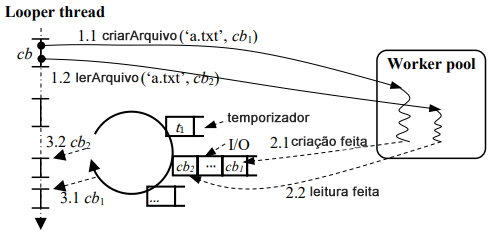
\includegraphics[width=0.8\textwidth]{images/pt-br/eda-arch-nodejs.png}
\label{fig:nodejs_eda_model}

Fonte: Adaptado de \cite{BUGS}.
\end{figure}

Na arquitetura orientada a eventos da plataforma do \textit{Node.JS} (\autoref{fig:nodejs_eda_model}), 
o fluxo de processamento de eventos da primeira etapa é realizada pelo \textit{loop thread}, 
buscando um evento no \textit{event loop} e, caso sua \textit{callback} não possa ser executada na mesma, ocorre
a transferência para a \textit{worker pool}, registrando uma nova \textit{callback} associada. 
Ainda, é possível observar este comportamento nas etapas 1.1 e 1.2, onde as ações de criação e leitura de 
um arquivo são transferidas à \textit{worker pool}, visto que são operações custosas e bloqueantes. Dada 
a transferência, a \textit{thread} principal permanece não-bloqueada e pode continuar seu processamento. 
Dentro da \textit{worker pool}, novas \textit{threads} podem ser criadas para realizar a execução das operações
assíncronas de I/O e, ao término, os eventos serão inseridos na fila específica para I/O (\textit{Node.JS} 
possui sete filas de eventos para diferentes tipos, sendo eles: temporizador, I/O, pendente, ocioso, preparação, 
verificação e fechamento \cite{NODEEVENTLOOP}). As etapas 2.1 e 2.2 representam este comportamento.
Por fim, a \textit{loop thread} busca estes novos eventos na fila e executa suas 
\textit{callbacks} (etapas 3.1 e 3.2) \cite{BUGS}.


\subsection{EDA \textit{vs.} OTPC}

A abordagem EDA, descrita na seção anterior, realiza multiplexação de uma única \textit{thread} para processar 
as requisições dos clientes, reduzindo, dessa forma, o consumo de recursos de máquina. 
A arquitetura de \textit{multithreading}, abordagem tradicional de aplicações \textit{web}, por sua vez, baseia-se
no conceito de uma \textit{thread} por cliente (\textit{One Thread Per Client}, OTPC), ou seja, cada requisição
recebida pelo servidor é atribuida à uma nova \textit{thread} para processamento isolado dos clientes, reduzindo
problemas relacionados à interferências. Contudo, cada requisição recebida resulta em sobrecarga no uso de
recursos de máquina e em trocas de contexto \cite{JGD}. Dessa forma, os custos computacionais aumentam
à medida que novos clientes realizam suas requisições, fazendo com que os sistemas limitem o número máximo de
\textit{threads} e, consequentemente, bloqueiem a escalabilidade do servidor \cite{ZRHR}.


\subsection{\textit{Stream}}

As \textit{streams} representam uma das mais importantes estruturas na plataforma do \textit{Node.JS}, por motivos
como aumento em desempenho e eficiência, possibilidade de criação de códigos elegantes e pela sua compatibilidade
no modelo da arquitetura orientada a eventos do \textit{Node.JS} \cite[p. 119]{MARIO}. Oferecem uma interface facilitada 
para leitura, gravação e transformação de dados, de forma que é possível realizar encadeamento 
entre estas operações para processá-los e, se necessário, transformá-los. Além dessas, essa estrutura está 
relacionada com os eventos, visto que utilizam destes para enviar notificações aos consumidores 
quando os dados estão prontos para consumo ou quando o processamento chegou ao fim \cite[p. 28]{DIOGORESENDE}.

O modelo da arquitetura baseada em eventos do \textit{Node.JS} aumenta a eficácia no uso das \textit{streams}, visto que,
em plataformas baseadas em eventos, a maneira mais eficiente para tratamento de I/O é com processamento em tempo real.
Dessa forma, a aplicação irá consumir os dados de entrada a medida que estes estão disponíveis, e o envio dos dados
de saída será de acordo com o ritmo de produção da aplicação \cite[p. 119]{MARIO}.

As \textit{streams}, além das características apresentadas, são utilizadas em problemas que não apresentam soluções tecnicamente
possíveis com outras interfaces presentes na plataforma do \textit{Node.JS}, como, por exemplo, a leitura de 
arquivos suficientemente grandes com funções que retornam um \textit{buffer} ao término da leitura completa. Arquivos com 
centenas de \textit{megabytes} ou até mesmo \textit{gigabytes}, precisariam ser carregados em um único 
\textit{buffer}, o que torna esse cenário inviável, visto que a aplicação ficaria sem memória, ainda mais ao 
imaginarmos cenários de aplicações \textit{web} onde seria necessário realizar diversas leituras simultâneas.
Ademais, o V8 (mecanismo presente no \textit{Node.JS} responsável pela execução de códigos \textit{JavaScript} \cite{NODEV8}) impõe 
um limite máximo de, aproximadamente, 1 GB para \textit{buffers}, o que explica a impossibilidade técnica para problemas 
desta natureza \cite[p. 122]{MARIO}.

\subsection{\textit{Buffer}}

Os \textit{buffers}, no \textit{Node.JS}, são objetos especiais utilizados para armazenamento e processamento 
de dados binários, o que não seria possível operando com tipos primitivos do \textit{JavaScript} como, por exemplo,
\textit{strings}, visto que estas são codificadas em \textit{Unicode} \cite[p. 29]{DIOGORESENDE}.

Além da possibilidade de manipulação de dados binários e da facilidade em leituras e escritas de números representados
com estruturas de tamanhos e formatos (\textit{big-endian} e \textit{little-endian}) diferentes, os \textit{buffers} são uma importante estrutura na plataforma do \textit{Node.JS} em relação à arquitetura
orientada a eventos, dada a compatibilidade binária existente entre os principais módulos da plataforma que 
utilizam estes nos eventos de dados. Dessa forma, é possível que arquivos sejam transmitidos ao cliente de maneira 
simplificada, ao modo que esta operação se resume ao encadeamento de \textit{streams} com a troca de 
\textit{buffers} entre cliente e servidor \cite[p. 29]{DIOGORESENDE}.


\subsection{\textit{Cluster}}

A técnica de clusterização pode ser utilizada para escalar horizontalmente um servidor em uma única máquina,
criando processos filhos, chamados de \textit{workers}, que executam de forma concorrente e compartilham uma mesma porta.
O \textit{Node.js} fornece o módulo de \textit{cluster} para permitir a execução de várias instâncias de aplicações na
mesma máquina. Esse módulo é semelhante ao módulo \textit{child\textunderscore process}, também nativo do \textit{Node.js},
que fornece o método \textit{fork} para criar subprocessos, sendo a principal diferença entre os dois módulos
um mecanismo adicional que permite o roteamento de solicitações recebidas, distribuindo-as entre as instâncias
criadas. O roteamento das solicitações é feito usando o algoritmo \textit{round-robin}, que encaminha a solicitação
para o próximo processo filho disponível, em uma ordem circular. \cite[p. 76]{DISTRIBUTEDNODE}.

\section{Trabalhos relacionados}

Nesta seção, serão discutidos trabalhos relacionados que abordaram o desempenho e o consumo de recursos 
em sistemas \textit{web}, particularmente aqueles desenvolvidos com \textit{Node.js}. Esses estudos ajudam a contextualizar 
o presente trabalho e fornecem insights valiosos sobre otimizações e estratégias para lidar com demandas 
intensas de dados.

Um estudo anterior \cite{CLUSTERTCC} se concentrou na melhoria do desempenho em sistemas \textit{web} por meio de atualizações 
de código e da implementação do módulo de \textit{cluster} no ambiente \textit{Node.js}. Os resultados indicaram melhorias 
significativas, demonstrando a eficácia de distribuir a carga de trabalho entre processos paralelos usando a 
técnica de \textit{clustering}. Essa abordagem se alinha diretamente com o nosso objetivo de entender como o consumo 
de recursos afeta o desempenho em sistemas \textit{web} com \textit{Node.js}, especialmente sob alta demanda de dados.
Da mesma forma, \cite{CLUSTERTCC} explorou otimizações em funções de cálculo de custos em sistemas 
semelhantes. Observou-se que melhorias substanciais foram alcançadas ao aprimorar a eficiência na 
iteração de matrizes e no gerenciamento de memória. Esses resultados ressaltam a importância de abordar o 
processamento intensivo de dados para melhorar o desempenho geral do sistema, uma consideração crucial em 
nossa investigação sobre sistemas \textit{web} de alta demanda.

Além das melhorias já exploradas, o trabalho também apontou oportunidades não 
investigadas, como a compilação AOT (\textit{Ahead of Time}) e a implementação de processos dedicados em segundo 
plano. Essas estratégias oferecem caminhos adicionais para otimização e merecem consideração em futuras 
iterações do projeto. Além disso, a implantação segura de técnicas como o clustering foi destacada como uma 
consideração crítica, enfatizando a necessidade de garantir a estabilidade e a segurança do sistema em produção.

Outro estudo anterior por \cite{NODEJVERSUSIIS} realizou uma comparação e avaliação do desempenho entre \textit{Node.js}, a mais recente 
tecnologia, e o servidor \textit{IIS}, por meio de testes objetivos e sistemáticos. Os resultados 
destacaram que o \textit{Node.js} apresenta um bom desempenho em relação ao servidor tradicional \textit{IIS} na 
execução de tarefas intensivas de I/O. Além disso, o estudo sugeriu que o \textit{Node.js} é preferencialmente utilizado 
em situações de I/O intensivo, em vez de serviços intensivos em CPU. Ao observar os resultados de desempenho em 
termos de \textit{throughput}, o \textit{Node.js} emergiu como uma tecnologia amplamente adotada por muitas organizações, 
especialmente devido às suas vantagens em cenários de I/O intensivo.

Esses estudos não apenas contribuem para o entendimento do contexto em que o presente trabalho se insere, 
mas também fornecem um ponto de partida sólido para nosso próprio estudo sobre o desempenho em função 
do consumo de recursos em sistemas \textit{web} desenvolvidos com \textit{Node.js}. Ao avaliar suas metodologias e 
resultados à luz de nossos objetivos, podemos identificar lacunas e direções promissoras para nossa 
pesquisa, ampliando assim o conhecimento sobre estratégias de otimização e gerenciamento de recursos 
em ambientes de alta demanda.


\section{Metodologia}

A metodologia aplicada apresenta caráter semi-experimental, qualitativo
e escopo exploratório, para análise do desempenho de sistemas \textit{web} baseados em \textit{Node.JS} 
quando será gerada uma condição de tráfego de fluxo intenso de dados,
com tamanhos de arquivo na ordem de \textit{gigabytes}.

O estudo será realizado em um ambiente controlado, onde serão desenvolvidos cenários de teste com diferentes 
implementações de arquitetura para a resolução do problema de envio de dados, a fim de aferir métricas de desempenho do servidor, 
como o consumo de memória \textit{RAM}, \textit{throughput} (quantidade de requisições processadas por unidade 
de tempo - vazão) e a média do tempo de resposta do servidor, que se refere ao tempo total que uma requisição leva
para ser completa. Uma implementação utilizará uma arquitetura não escalável e não 
pensada para o caso específico de transferência de um grande volume de dados, e outra aplicará técnicas focadas na 
manipulação de maiores volumes de dados.

Por meio da análise das implementações a serem definidas em seguida, procura-se salientar a melhora de performance,
principalmente no que diz respeito à múltiplas requisições paralelas, visto que uma implementação síncrona de operações
\textit{I/O} causa o bloqueio da \textit{thread} principal do \textit{Node.js}, não permitindo processamento paralelo.


\subsection{Implementações}

Serão abordadas, nesta seção, as implementações cruciais que foram desenvolvidas e 
otimizadas para avaliar e aprimorar o desempenho no ambiente \textit{Node.js}. Compreendendo a 
importância de alcançar um desempenho eficiente em aplicações \textit{web} com consumo de dados na ordem
de \textit{gigabytes}, foram adotadas estratégias e técnicas para maximizar a capacidade de 
processamento, minimizar os gargalos de execução e otimizar o consumo de recursos. 

\begin{lstlisting}[caption={Código base para um servidor \textit{Node.JS}}, label=cod:base]
	createServer(async (request, response) => {
		let startTime = -1;
  	const requestId = randomUUID();

		if (request.method === "OPTIONS") {
			response.writeHead(204, headers);
			response.end();
			return;
		}

		request.once("close", () => {
			saveRequestMetrics({
				requestId,
				server: "sync",
				startTime,
				endTime: performance.now(),
			});
		});

		response.writeHead(200, headers);

		try {
			startTime = performance.now();
			const { size } = await stat(filename);
			console.log(
				`${format(new Date(), "dd/MM/yyyy HH:mm:ss")} ${requestId} Processing: `,
				`${byteSize(size)}`
			);

			{ ... }
		} catch (error) {
			console.error(`Error at server: ${error.message}`);
			response.statusCode = 500;
			response.end("Internal Server Error");
		}
	})
  .listen(PORT)
  .on("listening", () => console.log(`server is running at ${PORT}`));
\end{lstlisting}

O Código~\ref{cod:base} apresenta a estrutura base para criação de servidores simples usando a 
plataforma do \textit{Node.JS}. Para tal, é utilizada a função \textit{createServer} do módulo nativo \textit{http}.
A sua \textit{callback} recebe os objetos de requisição e resposta para tratamentos como definição de cabeçalhos, leitura
de valores de entrada e escrita de valores de saída. Dessa forma, o servidor para este estudo irá responder à chamadas
realizadas no caminho raíz da aplicação, em determinada porta arbitrária.

A primeira implementação realizada, ilustrada no Código~\ref{cod:sync}, realiza a leitura do arquivo de 1.65 GB
de forma síncrona utilizando chamadas do módulo \textit{fs} (\textit{file system}), ou seja, todo o conteúdo será
inserido dentro de um único \textit{buffer} e retornado assim que a operação esteja concluída. Este trecho de código
deve ser inserido dentro do servidor previamente implementado no Código~\ref{cod:base}.

\begin{lstlisting}[caption={Implementação da leitura do arquivo de forma síncrona}, label=cod:sync]
	const data = fs.readFileSync(filename);
	response.end(data);
\end{lstlisting}

O Código~\ref{cod:async} apresenta a implementação inicial para a leitura do arquivo de 1.65 GB de forma assíncrona,
onde o conteúdo será processado sob demanada em pequenas porções - denominadas \textit{chunks}. Para tal, é utilizada
a função \textit{createReadStream} presente no módulo \textit{fs} (nativo da plataforma do \textit{Node.JS}) para
criar um \textit{stream} de leitura. Este trecho de código deve ser inserido dentro do servidor previamente 
implementado no Código~\ref{cod:base}.

O código apresenta uma sequência de operações que visam processar dados de um arquivo \textit{CSV} e 
transformá-los em formato \textit{JSON} (\textit{JavaScript object notation}). Através de uma abordagem baseada 
em fluxos de dados, o código executa alguma etapas de processamento. Após a criação da \textit{stream}, 
os dados do arquivo são canalizados em um processo de 
transformação usando o método \textit{pipeThrough} duas vezes. A primeira envolve a 
conversão dos dados \textit{CSV} em \textit{JSON}, através de uma biblioteca da comunidade (\textit{csvtojson}), 
selecionando apenas três propriedades escolhidas arbitrariamente. A conversão foi realizada a fim de facilitar
a manipulação dos dados no formato nativo da linguagem \textit{JavaScript}. O segundo processamento cria uma 
transformação personalizada, onde os dados \textit{JSON} são processados um a um. 
Para cada \textit{chunk} do arquivo, os campos são extraídos e usados para criar um novo objeto 
\textit{JSON} com os campos renomeados. Este processamento foi realizado apenas para demonstrar que, além de uma simples
transferência de dados, é possível realizar processos intermediários dentro do fluxo criado.

Para finalizar o processamento, a saída da transformação é canalizada para uma saída de uma resposta à requisição
\textit{HTTP}, realizada através do método \textit{pipeTo}. A opção \textit{signal} cria a possibilidade de 
cancelar a operação, o que é especialmente útil em cenários em que a mesma precisa ser interrompida. Todos os utilitários
usados para leitura (\textit{Readable}), escrita (\textit{Writable}) e transformação (\textit{Transform}) são ofertados
pelo módulo nativo \textit{stream} da plataforma do \textit{Node.JS}.

\begin{lstlisting}[caption={Implementação da leitura do arquivo de forma assíncrona}, label=cod:async]
	await Readable.toWeb(createReadStream(filename))
		.pipeThrough(
			Transform.toWeb(
				csvtojson({ headers: ["cord_uid", "sha", "publish_time"] })
			)
		)
		.pipeThrough(
			new TransformStream({
				async transform(chunk, controller) {
					const {
						cord_uid: cordUid,
						sha,
						publish_time: publishTime,
					} = JSON.parse(Buffer.from(chunk));

					const mappedData = {
						cordUid,
						sha,
						publishTime,
					};

					controller.enqueue(JSON.stringify(mappedData).concat("\n"));
				},
			})
		)
		.pipeTo(Writable.toWeb(response));
\end{lstlisting}

O Código~\ref{cod:async-cluster}, ainda, foi utilizado para a terceira versão do servidor, somando à técninca de leitura
assíncrona de arquivos com a clusterização, implementada a partir de módulo \textit{cluster}, nativo da plataforma
\textit{Node.JS}. É possível observar que o processo principal será responsável pela criação de processos filhos a partir
do comando \textit{fork}, criando uma quantidade de processos referente ao número de núcleos de processamento presentes
no processador da máquina. Os processos filhos, por sua vez, serão responsáveis pela instanciação de um servidor com 
a implementação de leitura assíncrona, igualmente como apresentada no Código~\ref{cod:async}.

\begin{lstlisting}[caption={Implementação da técnica de clusterização}, label=cod:async-cluster]
	if (cluster.isPrimary) {
		const numCPUs = os.cpus().length;

		for (let i = 0; i < numCPUs; i += 1) {
			cluster.fork();
		}

		console.log(`Number of workers: ${Object.keys(cluster.workers).length}`);

		cluster.on("exit", (worker) => {
			console.log(`Worker ${worker.process.pid} died`);
			cluster.fork();
		});
	} else {
		{ ... }
	}
\end{lstlisting}


\subsection{Base de teste}

A base de dados utilizada para testes foi escolhida baseando-se em seu tamanho (ordem de \textit{gigabytes}) com
o objetivo de garantir resultados significativos para o estudo. Escolheu-se uma base com dados estruturados com o 
objetivo de exemplificar a aplicação prática do processamento intermediário no processo de transferência. 
Ao optar por essa abordagem, busca-se enfatizar a necessidade de ir além da mera transferência direta, 
incorporando etapas de processamento que permitam aprimorar a integridade e utilidade dos dados no contexto de destino.

O arquivo final utilizado apresenta um tamanho de 1.65 GB, sendo do formato \textit{CSV} (\textit{comma separated values}) 
com 19 propriedades separadas em colunas. A extração foi realizada da base 
\textit{CORD-19: COVID-19 Open Research Dataset} \cite{BASE}. Destaca-se que a escolha foi realizada a partir 
de fontes confiáveis e respeitando os critérios éticos e legais. O tratamento das informações contidas será de 
acordo com as técnicas e métodos descritos nas seções subsequentes deste trabalho.


\subsection{Definição dos cenários de teste}

% metodologia - começar com poucas requisições e ir aumentando

Serão definidos três cenários de teste para avaliar o desempenho das implementações quando confrontadas
com uma transferência de um volume de dados de 1.65 \textit{gigabytes}. Os cenários de teste serão 
nomeados da seguinte forma:

\begin{enumerate}[a)]
\item Cenário 1: Implementação com arquitetura não específica para transferências da ordem de \textit{gigabytes}, 
ou seja, realização da leitura de arquivos de forma síncrona (Código~\ref{cod:sync}).
\item Cenário 2: Implementação com arquitetura escalável para transferências da ordem de \textit{gigabytes}, 
utilizando métodos da arquitetura baseada em eventos para ler arquivos de forma assíncrona (Código~\ref{cod:async}).
\item Cenário 3: Implementação com arquitetura escalável para transferências da ordem de \textit{gigabytes}, 
utilizando métodos da arquitetura baseada em eventos para ler arquivos de forma assíncrona somada à utilização de
\textit{clusters} (Código~\ref{cod:async-cluster}).
\end{enumerate}


\subsection{Construção do ambiente de teste}

Será configurado um ambiente de teste composto por uma aplicação servidor, com o intuito de registrar e avaliar as métricas como consumo
de memória \textit{RAM} e \textit{CPU}, \textit{throughput}, que se refere à quantidade de requisições feitas à aplicação por unidade de tempo,
e a média do tempo tempo de resposta do servidor nos três cenários propostos. 
O servidor de aplicação será baseado em \textit{Node.JS}, utilizando a versão 20.3.0. A aplicação será executada em uma máquina
com 24 \textit{gigabytes} de memória \textit{RAM} e um processador com 4 núcleos.

Para automatizar o envio de requisições ao servidor em diferentes cenários, 
foi desenvolvido um \textit{script shell}. Esse \textit{script} permite configurar a quantidade de 
requisições e automatiza o processo de envio de solicitações \textit{HTTP}. O Código~\ref{cod:shelltest} 
apresenta a configuração adotada em que são enviadas dez solicitações ao servidor. Para tornar o ambiente de 
teste mais realista, definiu-se a quantidade de solicitações enviadas simultaneamente, 
utilizando a opção \textit{-P}, com a quantidade de núcleos disponíveis da máquina executante (obtido com \textit{nproc}), 
da ferramenta \textit{xargs}, que permite a execução de comandos em lote. O envio 
das requisições é realizado por meio do comando \textit{curl}, que especifica o caminho e o método \textit{HTTP} apropriado.
Em resumo, serão enviadas quatro requisições ao mesmo tempo ao servidor até que se complete a quantidade total de solicitações.

\begin{lstlisting}[caption={\textit{Script} para disparo de requisições}, label=cod:shelltest]
	seq 1 10 | xargs -Iname -P $(nproc)  curl -X GET "http://localhost:${PORT}"
\end{lstlisting}


\subsection{Coleta e análise de dados}

Os indicadores de desempenho a serem coletados e analisados para cada uma das implementações, durante a transferência
dos dados contidos na base previamente citada serão: Uso de memória \textit{RAM}, uso de \textit{CPU}, \textit{throughput}
e a média do tempo de resposta do servidor.

O Código~\ref{cod:analytics} demonstra o \textit{script} utilizado para calcular as métricas \textit{throughput} e 
média do tempo de resposta do servidor. Para ambas, faz-se necessário definir a soma dos tempos de processamento de
todas as solicitações respondidas pelo servidor, somada à conversão do tempo em milissegundos para minutos.

\begin{lstlisting}[caption={Implementação do cálculo das métricas \textit{throughput} e média do tempo de resposta}, label=cod:analytics]
	const timeProcessingInSeconds =
    data.requests.reduce(
      (acc, current) => acc + (current.endTime - current.startTime),
      firstRequest.endTime - firstRequest.startTime
    ) / 1000;

  const analytics = {
    throughput: getFormattedMetric({
      value: numRequests / timeProcessingInSeconds,
      unity: "req/sec",
    }),
    avg: getFormattedMetric({
      value: timeProcessingInSeconds / numRequests,
      unity: "s",
    }),
  };
\end{lstlisting}

O \textit{throughput} e a média do tempo de resposta do servidor serão coletadas com código apresentado anteriormente.
Os dados necessários para o cálculo destas duas métricas serão armazenados em arquivos para análise após o fim de uma 
bateria de testes. Para ambos, faz-se necessário a captura do tempo de ínicio de uma requisição
e o tempo de fim da mesma. Estas duas variáveis serão obtidas utilizando
o módulo nativo \textit{perf\textunderscore hooks} da plataforma \textit{Node.JS}. 
O método \textit{now} deste módulo retorna o valor em milissegundos e será invocado no ínicio da 
\textit{callback} que trata as requisições do servidor, e, no evento de 
fechamento destas, o valor de ínicio, o valor de tempo atual e
uma identificação única da requisição serão armazenados em um arquivo \textit{JSON}. Após o encerramento do servidor, será 
possível, utilizando a soma da diferença dos tempos de início e fim de cada requisição, e a quantidade de requisições realizadas, calcular o 
\textit{throughput}, que terá a unidade requisições por minuto. Para o cálculo da média simples de tempo de resposta do servidor, 
as mesmas variáveis serão utilizadas, desta maneira, o valor pode ser calculado dividindo a diferença entre o tempo de fim e o 
tempo de início pelo número de requisições e somando o resultado.

O Código~\ref{cod:monit_single} foi implementado com o objetivo de executar o servidor e armazenar, em tempo real,
as métricas de uso de recursos de máquina, como consumos de memória \textit{RAM} e \textit{CPU}. Os valores 
são obtidos através da ferramenta \textit{ps} (relatório dos processos atuais), buscando através do 
\textit{PID} (\textit{process identifier}, identificador de processo). Os valores são salvos em tempo real em um arquivo 
\textit{CSV} a cada segundo (\textit{sleep 1}). O valor de consumo de memória \textit{RAM} é salvo após uma divisão por 1024, 
para que o mesmo seja convertido para \textit{megabytes}. 

\begin{lstlisting}[caption={\textit{Script} para monitrar processos \textit{single thread}}, label=cod:monit_single]
	node "$SERVER_FILE_NAME" &
	node_pid=$!

	while ps -p $node_pid > /dev/null; do
		timestamp=$(date +'%Y-%m-%d %H:%M:%S')
		usage_info=$(ps -p $node_pid -o rss,%cpu --no-headers)

		if [ -n "$usage_info" ]; then
			rss_mb=$(echo "$usage_info" | awk '{printf "%.2f", $1/1024}')
			cpu_usage=$(echo "$usage_info" | awk '{printf "%.2f", $2}')
			echo "$timestamp;$rss_mb;$cpu_usage" >> "$LOG_DIRECTORY/$LOG_FILE"
		else
			echo "Processo Node.js não encontrado."
			exit 1
		fi

		sleep 1
	done
\end{lstlisting}

O código anterior corresponde ao monitoramento do servidor nas arquiteturas com apenas um processo. Para o cenário
com \textit{clusters}, onde serão criados processos filhos, faz-se necessário uma adaptação 
demonstrada no Código~\ref{cod:monit_multi}. Neste, são recuperados os identificadores dos processos filhos 
a partir da ferramenta \textit{pgrep}, para que seja possível iterelá-los e monitorá-los individualmente, 
criando um arquivo de saída para cada.

\begin{lstlisting}[caption={\textit{Script} para monitrar processos \textit{multi thread}}, label=cod:monit_multi]
	worker_pids=$(pgrep -P $node_pid)
	for worker_pid in $worker_pids; do
		{...}
	done
\end{lstlisting}

Os gráficos referentes ao consumo de recursos de máquina, como \textit{RAM} e \textit{CPU}, são
gerados automaticamente a partir dos \textit{scripts} em \textit{Python}, como mostra o Código~\ref{cod:base_python}.
Os arquivos com o monitoramento em tempo real são lidos com o uso da biblioteca \textit{Pandas}, e
as figuras são geradas com o uso da biblioteca \textit{Matplotlib}.

\begin{lstlisting}[caption={\textit{Script} base em \textit{Python} para geração de gráficos.}, label=cod:base_python]
	def run(server, contentFileName, id=None):
		BASE_PATH = os.path.abspath(f"../server/tmp/{server}")

		df = getData(
			fileName=f"{BASE_PATH}/{contentFileName}"
		)

		generateFig(
			title="Gráfico Tempo X Consumo de RAM",
			x_label="Tempo",
			y_label="Memória (MB)",
			fileName=f"{BASE_PATH}/memory_usage{f'_{id}' if id is not None else ''}.png",
			x=df["timestamp"],
			y=df["memory"]
		)

		generateFig(
			title="Gráfico Tempo X Consumo de CPU",
			x_label="Tempo",
			y_label="CPU (%)",
			fileName=f"{BASE_PATH}/cpu_usage{f'_{id}' if id is not None else ''}.png",
			x=df["timestamp"],
			y=df["cpu"]
		)
\end{lstlisting}

Para a arquitetura com utilização de \textit{clusters}, faz-se necessária a criação de gráficos exclusivos aos processos
filhos. Para atender a este objetivo, adequou-se o \textit{script} como mostra o Código~\ref{cod:multi_python} para, 
inicialmente, realizar uma leitura de todos os arquivos de monitoramento do servidor desta arquitetura em específico.

\begin{lstlisting}[caption={Geração dos gráficos para servidor com arquitetura de \textit{cluster}}, label=cod:multi_python]
	csv_files = [f for f in os.listdir(f"{BASE_PATH}") if f.endswith('.csv')]

	for index, file in enumerate(csv_files):
		run(
			contentFileName=file,
			server=server,
			id=index
		)
\end{lstlisting}

O monitoramento do servidor é realizado desde sua inicialização até que ocorra uma interrupção. Para que seja possível uma
análise correta em relação ao tempo no qual este recebeu as requisições, faz-se necessário adaptações nos códigos para
que seja marcado os tempos de ínicio de fim da bateria de solicitações. O Código~\ref{cod:analytics_startend}, executado
ao mesmo tempo que o Código~\ref{cod:analytics}, demonstra a recuperação dos valores de ínicio de fim da bateria de
requisições, através de operações simples para busca dos valores de máximo e mínimo, fazendo com que estes sejam
gravados no mesmo arquivo de resultados.

\begin{lstlisting}[caption={Recuperação dos valores de início e fim da bateria de solicitações.}, label=cod:analytics_startend]
	const start =
    data.requests.length > 0
      ? data.requests.reduce(
          (acc, current) => (current.startTime < acc ? current.startTime : acc),
          data.requests[0].startTime
        )
      : startTime;

  const end =
    data.requests.length > 0
      ? data.requests.reduce(
          (acc, current) => (current.endTime > acc ? current.endTime : acc),
          data.requests[0].endTime
        )
      : endTime;
\end{lstlisting}

O Código~\ref{analytics_startend:fig} demonstra o uso das informações de início de fim da bateria de requisições para
criação dos gráficos. Esses valores (em milissegundos) são adicionados ao primeiro valor do arquivo de monitoramento
(valor o qual diz respeito ao instante em que o servidor foi iniciado), para que seja possível marcar esses valores no 
gráfico com pontos específicos. Posteriormente, são recuperados os valores de uso de \textit{CPU} e \textit{RAM} referentes
a estes tempos.

\begin{lstlisting}[caption={Recuperação das coordenadas de início e fim da bateria de solicitações.}, label=cod:analytics_startend:fig]
	end = -1
  start = -1

  with open(f"{BASE_PATH}/requests.json", "r") as json_file:
    content = json.load(json_file)
    start = content['start']
    end = content['end']

  target_start = df['timestamp'][0] + timedelta(milliseconds=start)
  target_end = df['timestamp'][0] + timedelta(milliseconds=end)

  start_time = min(df['timestamp'], key=lambda x: abs((x - target_start).total_seconds()))
  end_time = min(df['timestamp'], key=lambda x: abs((x - target_end).total_seconds()))

  start_usage = df[df['timestamp'] == start_time]
  end_usage = df[df['timestamp'] == end_time]
\end{lstlisting}

\section{Resultados e discussão}

Esta seção desempenha um papel central neste estudo, apresentando e analisando os resultados obtidos de 
acordo com a metodologia previamente descrita. Nesta seção, os dados coletados são examinados, suas implicações são interpretadas 
e as descobertas são discutidas à luz das questões de pesquisa estabelecidas. Os itens aqui apresentados representam o 
resultado de análises rigorosas e constituem uma contribuição significativa para a compreensão do tópico em questão.

A tabela \autoref{tab:metrics} apresenta a comparação dos valores de \textit{throughput} e tempo de resposta do servidor,
entre os três cenários estipulados, síncrono, assíncrono e assíncrono com uso de \textit{clusters}, quando confrontados
com 10 requisições, sendo quatro simultâneas, até atingir o total de requisições. Todas as requisições realizam a leitura
do arquivo de 1.65 \textit{gigabytes}. 

É evidente que, assim como
esperado, o cenário síncrono apresentou um \textit{throughput} inferior aos cenários assíncronos, ou seja, esta implementação
teve menos poder para lidar com requisições simultâneas. Também o tempo médio de resposta do servidor foi superior no caso
síncrono, estas duas métricas são justificadas devido à limitação de bloqueio da \textit{thread} principal do 
\textit{Node.js} durante uma leitura de arquivo síncrona, coisa que não ocorre em leituras assíncronas e permite que o
servidor execute tarefas paralelas. Comparando os dois métodos assíncronos, é também notável a melhora na performance da 
implementação que utiliza \textit{clusters} para obter mais poder de processamento paralelo, pois esta aproveita
os núcleos disponíveis do processador para que o servidor consiga atender à mais solicitações simultaneamente,
dando escalabilidade horizontal ao servidor.

\begin{table}[!h]
\centering
\caption{Métrica de tempo calculadas por arquitetura de servidor} 
\label{tab:metrics}
\begin{tabular}{|p{3cm}|p{3cm}|p{3cm}|p{3cm}|}
\hline
\textbf{Métrica} & \textbf{Síncrono} & \textbf{Assíncrono} & \textbf{Assíncrono com \textit{clusters}} \\
\hline
\textit{Throughput} (req/min) & 0.042 & 0.180 & 0.325\\
\hline
Média do tempo de resposta (min) & 24.064 & 5.565 & 3.079\\
\hline
\end{tabular}
\end{table}


A \autoref{fig:sync_memory_usage} apresenta o uso de memória \textit{RAM} da implementação síncrona,
durante o tempo de uma requisição para a transferência do arquivo de 1.65 \textit{gigabytes}. É 
possível notar o uso elevado de memória, com um pico de X \textit{megabytes}, assim como é observável
que a memória se mantém constante, isso ocorre pois o método síncrono lê o arquivo, que é constante,
por inteiro e o armazena na memória.

Também pode-se observar que mesmo ao término da leitura,
a memória \textit{RAM} utilizada não é desalocada imediatamente, ficando em um valor estável.
Isso ocorre porque na \textit{V8} do \textit{Node.js}, a contagem de referências é verificada periodicamente em um
processo chamado "ciclo", que pode pausar brevemente a execução do programa, isso requer memória 
adicional para o \textit{Garbage Collector}, portanto, o \textit{GC} é executado periodicamente,
fazendo com que o lixo (memória não utilizada) permaneça por mais tempo do que o necessário. \cite[p. 35]{DIOGORESENDE}


\begin{figure}[!h]
\centering
\caption{Síncrono: Uso de memória \textit{RAM} X tempo}
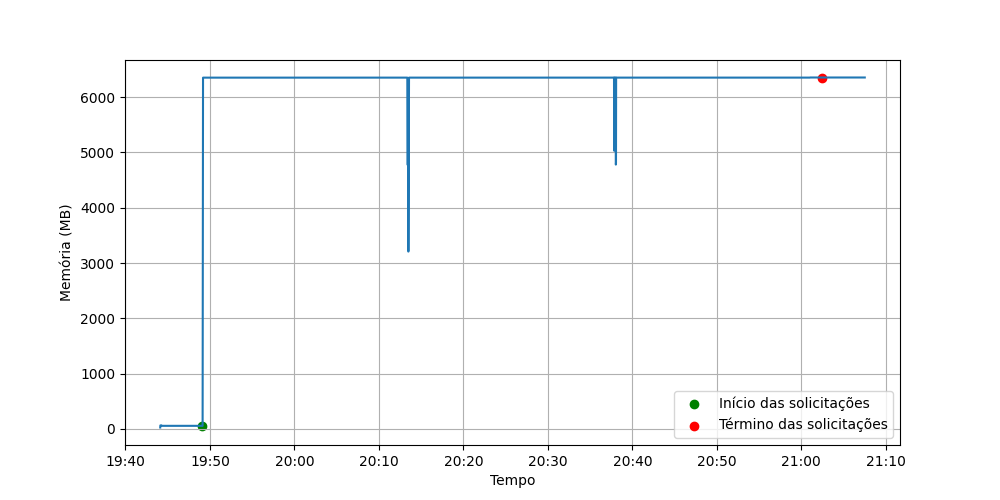
\includegraphics[width=0.8\textwidth]{images/pt-br/results/sync_memory_usage.png}
\label{fig:sync_memory_usage}

Fonte: Os Autores.
\end{figure}


Ao contrário da memória \textit{RAM} que inicia no menor valor, a \autoref{fig:sync_cpu_usage}
mostra que o \textit{CPU} tem um uso elevado na criação do servidor, mas que logo
cai para valores muito baixos até que receba uma requisição para o processamento do arquivo. 
Diferente da memória \textit{RAM}, o uso de \textit{CPU} cai uniformemente ao final 
do processamento dos dados.


\begin{figure}[!h]
\centering
\caption{Síncrono: Uso de \textit{CPU} X tempo}
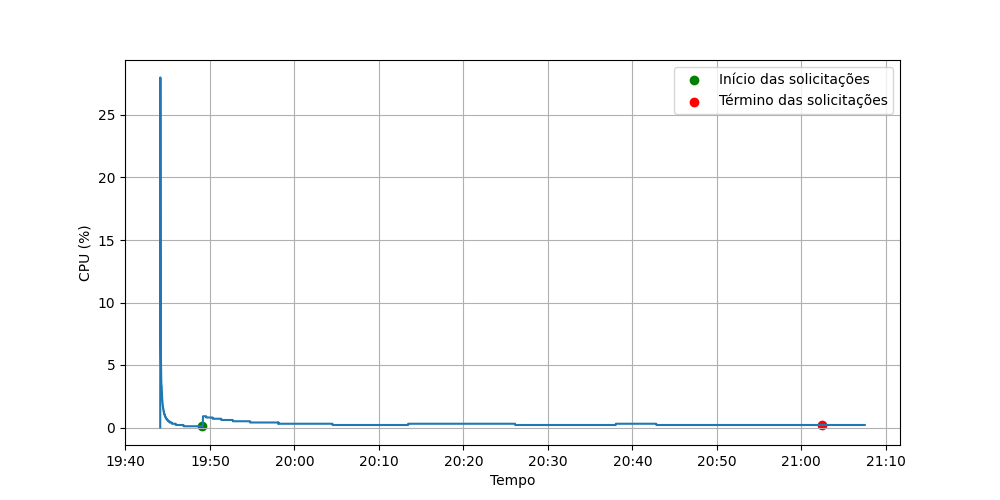
\includegraphics[width=0.8\textwidth]{images/pt-br/results/sync_cpu_usage.png}
\label{fig:sync_cpu_usage}

Fonte: Os Autores.
\end{figure}


Para o uso de memória \textit{RAM} da implementação assíncrona já é possível
notar uma grande diferença, esta implementação faz muito menos uso do recurso que
o método anterior, atingindo, aproximadamente, 200 \textit{megabytes} em seu pico
\autoref{fig:async_memory_usage}. O uso da memória no método assíncrono também se
difere do síncrono por não manter a memória constante, pois o método lê \textit{chunks}
que não necessariamente tem o mesmo tamanho, pois cada linha do arquivo pode ter um
tamanho diferente.


\begin{figure}[!h]
\centering
\caption{Assíncrono: Uso de memória \textit{RAM} X tempo}
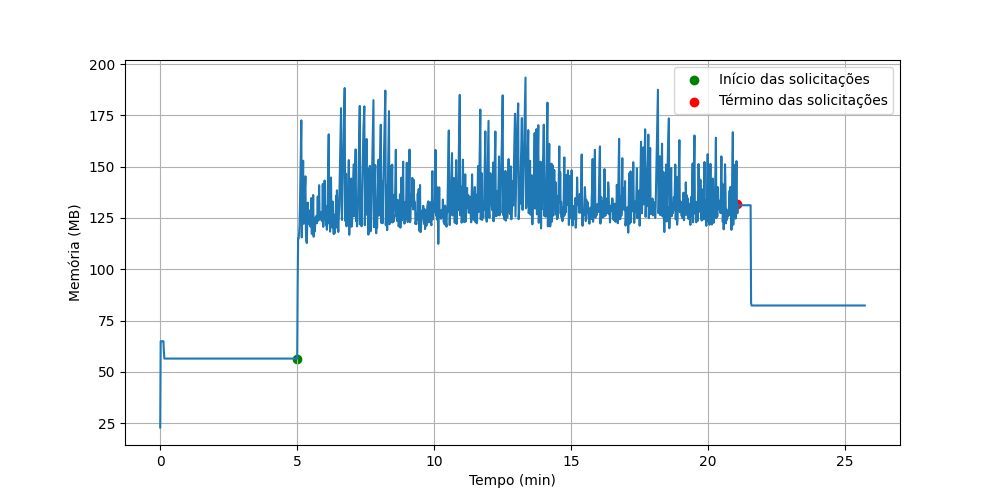
\includegraphics[width=0.8\textwidth]{images/pt-br/results/async_memory_usage.png}
\label{fig:async_memory_usage}

Fonte: Os Autores.
\end{figure}

Contudo, a responsabilidade é transferida para o \textit{CPU},
que apresenta um uso bem mais elevado e próximo ao 100\text{\%}, como é possível
observar na \autoref{fig:async_cpu_usage}

\begin{figure}[!h]
\centering
\caption{Assíncrono: Uso de \textit{CPU} X tempo}
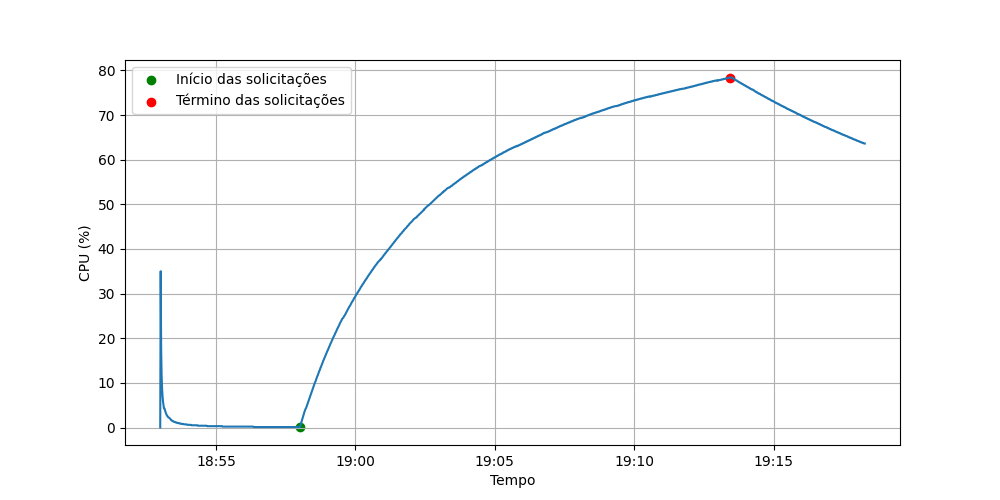
\includegraphics[width=0.8\textwidth]{images/pt-br/results/async_cpu_usage.png}
\label{fig:async_cpu_usage}

Fonte: Os Autores.
\end{figure}


A implementação assíncrona somada ao uso de \textit{clusters} teve os melhores resultados
em relação às métricas de \textit{throughput} e média de tempo de resposta do servidor,
como demonstrado na \autoref{tab:metrics}. Para o uso de memória \textit{RAM} 
(\autoref{fig:async-cluster_memory_usage_0}), esta implementação
apresentou os menores valores se analisarmos cada processo filho isoladamente, porém, se os
agregarmos, o uso deste recurso torna-se mais elevado que o da implementação assíncrona, mas
ainda assim menor que o da implementação assíncrona.


\begin{figure}[!h]
\centering
\caption{Assíncrono primeiro \textit{cluster}: Uso de memória \textit{RAM} X tempo}
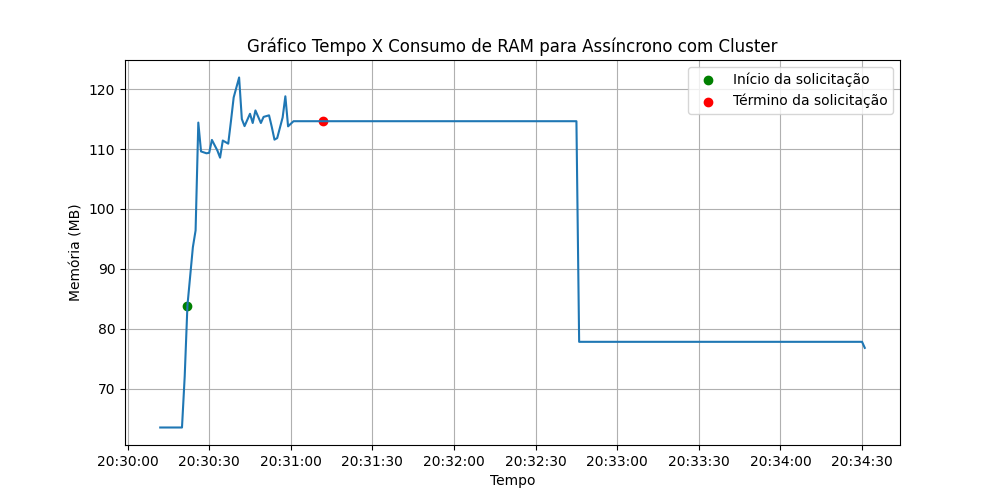
\includegraphics[width=0.8\textwidth]{images/pt-br/results/async-cluster_memory_usage_0.png}
\label{fig:async-cluster_memory_usage_0}

Fonte: Os Autores.
\end{figure}

O uso de \textit{CPU} \autoref{fig:async-cluster_cpu_usage_0} se comporta da mesma maneira
maneira, mantendo valores mais brandos se observado apenas um processo filho de forma isolada.
Nota-se que o consumo de recursos que cada processo filho utiliza a mais que o único processo
da implementação assíncrona, se traduz para a melhora das métricas de desempenho de 
\textit{throughput} e média de tempo de resposta do servidor.

\begin{figure}[!h]
\centering
\caption{Assíncrono primeiro \textit{cluster}: Uso de \textit{CPU} X tempo}
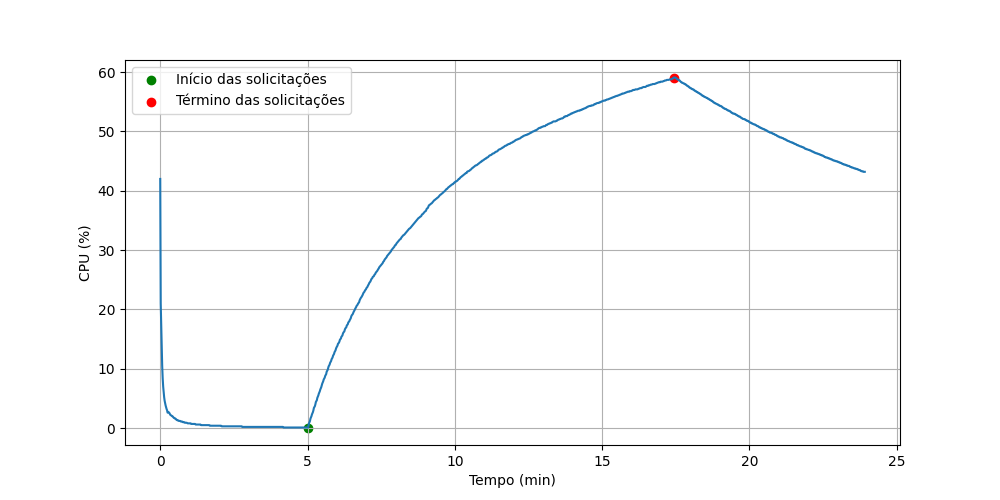
\includegraphics[width=0.8\textwidth]{images/pt-br/results/async-cluster_cpu_usage_0.png}
\label{fig:async-cluster_cpu_usage_0}

Fonte: Os Autores.
\end{figure}


Os gráficos apresentados da \autoref{fig:async-cluster_memory_usage_1} até a 
\autoref{fig:async-cluster_cpu_usage_3} mostram o uso de memória \textit{RAM}
e \textit{CPU} para os demais processos filhos da implementação assíncrona com o uso
de \textit{clusters}. Os dados são similares entre os quatro processos filhos e 
levam à mesma conclusão sobre o uso destes recursos da máquina.


\begin{figure}[!h]
\centering
\caption{Assíncrono segundo \textit{cluster}: Uso de memória \textit{RAM} X tempo}
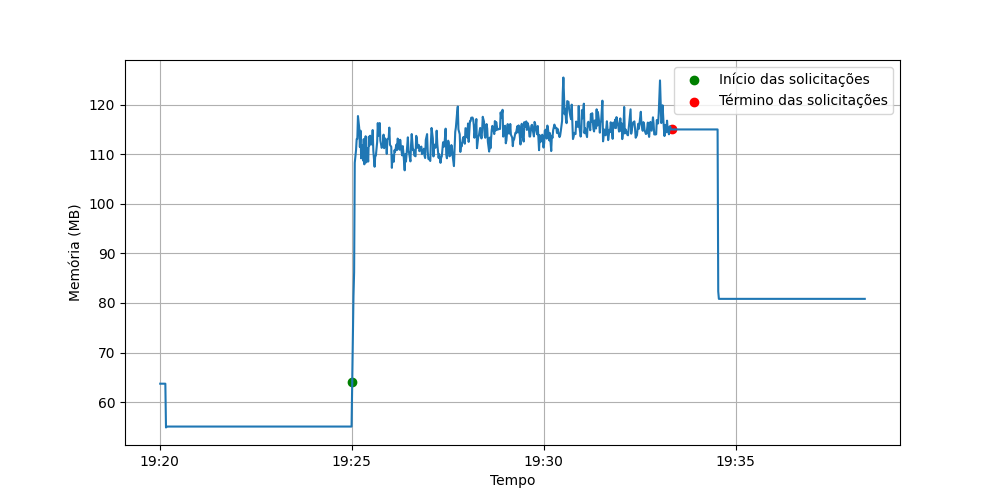
\includegraphics[width=0.8\textwidth]{images/pt-br/results/async-cluster_memory_usage_1.png}
\label{fig:async-cluster_memory_usage_1}

Fonte: Os Autores.
\end{figure}

\begin{figure}[!h]
\centering
\caption{Assíncrono segundo \textit{cluster}: Uso de \textit{CPU} X tempo}
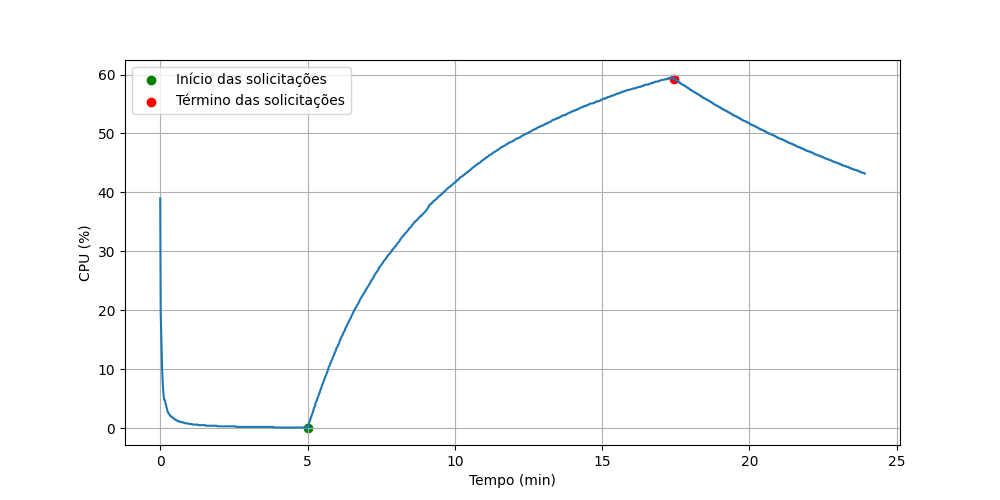
\includegraphics[width=0.8\textwidth]{images/pt-br/results/async-cluster_cpu_usage_1.png}
\label{fig:async-cluster_cpu_usage_1}

Fonte: Os Autores.
\end{figure}

%async-cluster_cpu_usage_2.png

\begin{figure}[!h]
\centering
\caption{Assíncrono terceiro \textit{cluster}: Uso de memória \textit{RAM} X tempo}
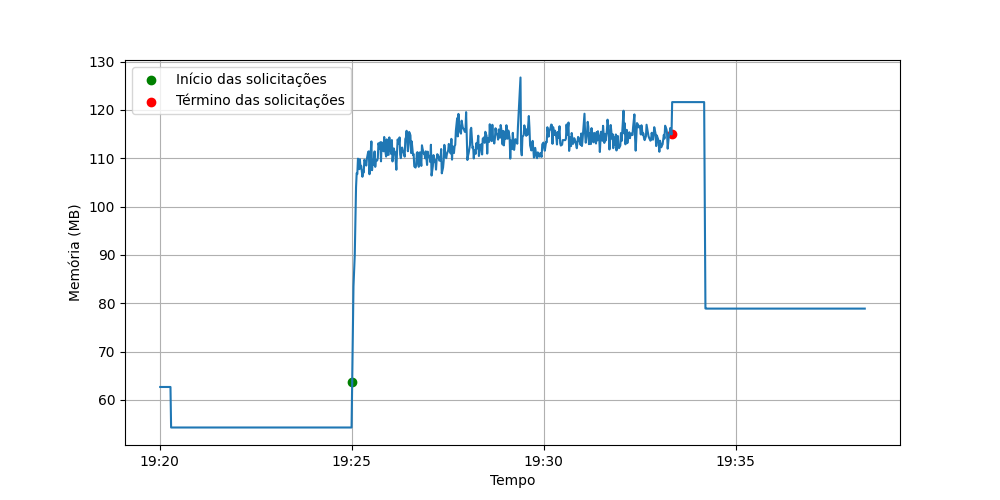
\includegraphics[width=0.8\textwidth]{images/pt-br/results/async-cluster_memory_usage_2.png}
\label{fig:async-cluster_memory_usage_2}

Fonte: Os Autores.
\end{figure}

\begin{figure}[!h]
\centering
\caption{Assíncrono terceiro \textit{cluster}: Uso de \textit{CPU} X tempo}
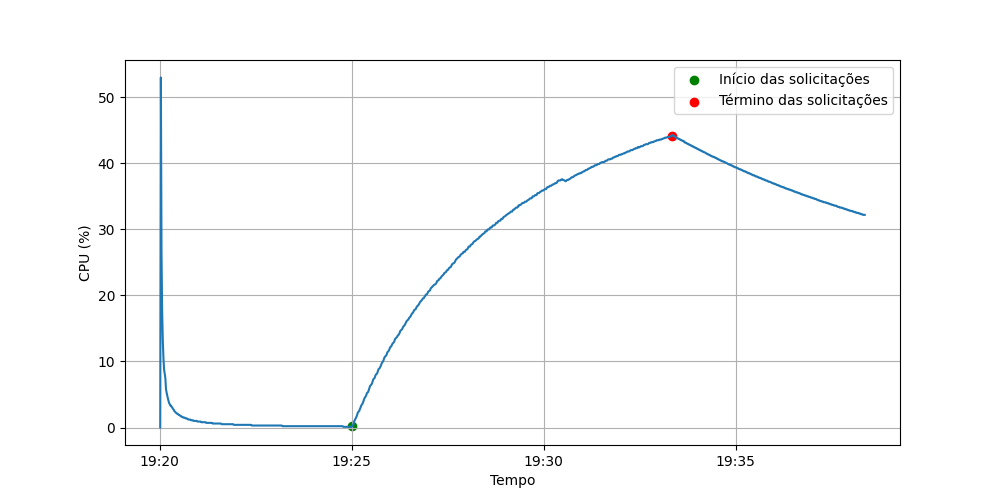
\includegraphics[width=0.8\textwidth]{images/pt-br/results/async-cluster_cpu_usage_2.png}
\label{fig:async-cluster_cpu_usage_2}

Fonte: Os Autores.
\end{figure}

%async-cluster_cpu_usage_3.png

\begin{figure}[!h]
\centering
\caption{Assíncrono quarto \textit{cluster}: Uso de memória \textit{RAM} X tempo}
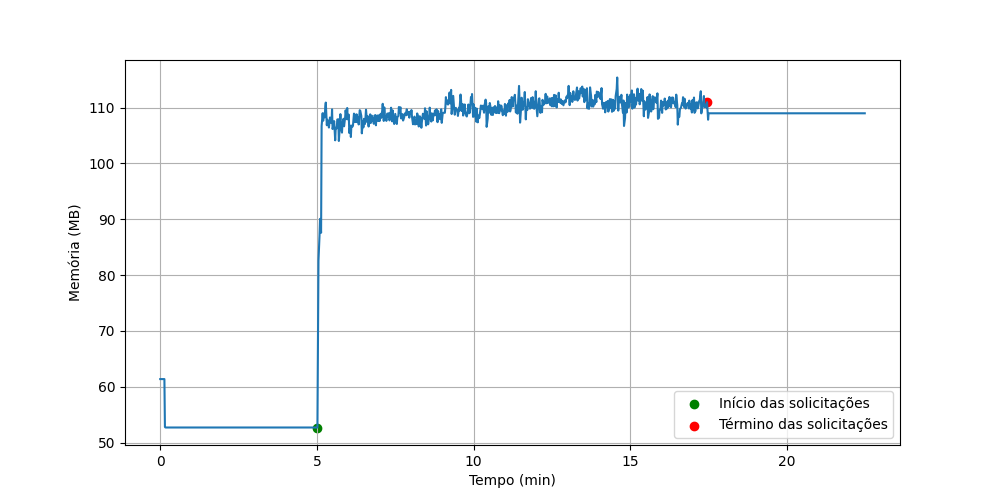
\includegraphics[width=0.8\textwidth]{images/pt-br/results/async-cluster_memory_usage_3.png}
\label{fig:async-cluster_memory_usage_3}

Fonte: Os Autores.
\end{figure}

\begin{figure}[!h]
\centering
\caption{Assíncrono quarto \textit{cluster}: Uso de \textit{CPU} X tempo}
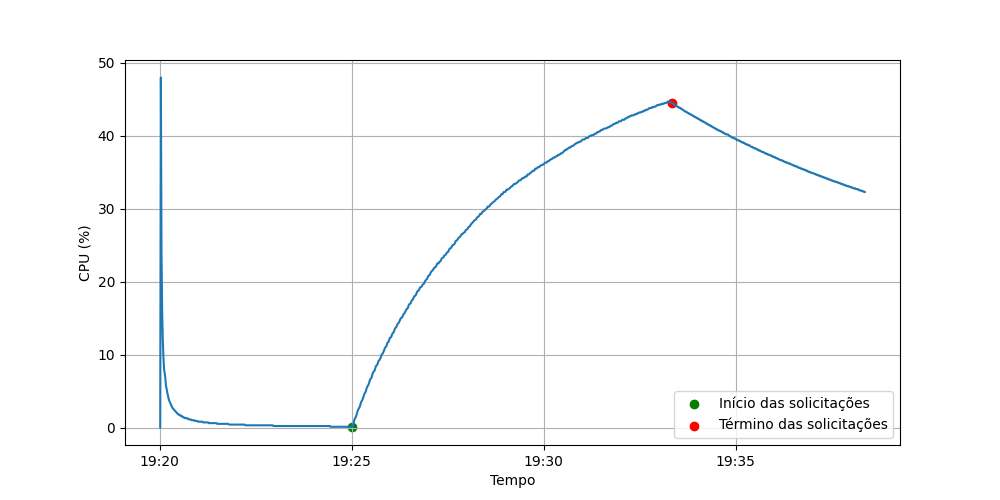
\includegraphics[width=0.8\textwidth]{images/pt-br/results/async-cluster_cpu_usage_3.png}
\label{fig:async-cluster_cpu_usage_3}

Fonte: Os Autores.
\end{figure}


Após análise das quatro métricas escolhidas, apresentadas por meio da tabela de comparações
entre os cenários e gráficos individuais destes, pode-se concluir que das três 
implementações, a que obteve pior desempenho e pior uso dos recursos, quando confrontada 
com a base de dados de 1.65 \textit{gigabytes}, foi a síncrona. O uso da memória \textit{RAM}
foi o mais elevado, e, mesmo assim, o cenário teve um desempenho pior em relação ao 
\textit{throughput} e média do tempo de resposta do servidor, demorando muito mais
para atender às requisições do que os outros cenários.


\section{Considerações finais}

Este estudo investigou o desempenho de sistemas web desenvolvidos com \textit{Node.js} em cenários com transferência de dados
na ordem de \textit{gigabytes}, considerando três abordagens diferentes de leitura de arquivos. Os resultados destacam
a importância da escolha da estratégia correta para operações de leitura em sistemas feitos com \textit{Node.js}.

Em resumo, a leitura síncrona de arquivos demonstrou ser ineficiente em situações de alta demanda, resultando em 
tempos de resposta insatisfatórios, e, quando confrontada com a leitura e transferência de um arquivo de 1.65 \textit{gigabytes},
apresentou um desempenho, no geral, ruim. Por outro lado, o método assíncrono se mostrou um caminho possível para a manipulção de um arquivo de
grandes proporções, mesmo consumindo recursos, ainda que reduzidos em relação à leitura síncrona, como é o caso do uso de
memória \textit{RAM}, este cenário demonstrou a possibilidade do \textit{Node.js} para tais casos. Ainda, a implementação 
de leitura assíncrona combinada com o uso de \textit{clusters} se destacou como a abordagem mais eficiente e escalável, otimizando 
significativamente o desempenho em cenários de alta concorrência, por realizar o processamento necessário de forma distribuída. 
É fundamental destacar um dos principais benefícios proporcionados pelo uso do método assíncrono, que é a capacidade de lidar 
com múltiplas solicitações concorrentes, ao contrário do método síncrono, o método assíncrono não impede a execução normal 
de outras instruções, permitindo que várias tarefas sejam processadas simultaneamente de forma eficiente.

\bibliographystyle{sbc}
\bibliography{referencias}

\end{document}